\section{Результаты измерений}
\[
    U_{\text{заж}} = 2180\pm10\;\text{В}
\]

\begin{table}[!ht]
    \centering
    \caption{ВАХ}
    \begin{tabular}{|l|l|}
\hline
$U,\;\text{В}$ & $I,\;\text{мА}$\\\hline
$34{,}30 \pm 0{,}10$ & $\left(528{,}7 \pm 1{,}5\right)\cdot 10^{-3}$\\\hline
$33{,}07 \pm 0{,}10$ & $\left(796 \pm 2\right)\cdot 10^{-3}$\\\hline
$32{,}25 \pm 0{,}10$ & $\left(1105 \pm 3\right)\cdot 10^{-3}$\\\hline
$31{,}70 \pm 0{,}10$ & $\left(1412 \pm 3\right)\cdot 10^{-3}$\\\hline
$31{,}05 \pm 0{,}09$ & $\left(1713 \pm 4\right)\cdot 10^{-3}$\\\hline
$28{,}03 \pm 0{,}08$ & $\left(2007 \pm 4\right)\cdot 10^{-3}$\\\hline
$23{,}62 \pm 0{,}07$ & $\left(2319 \pm 5\right)\cdot 10^{-3}$\\\hline
$21{,}11 \pm 0{,}06$ & $\left(2694 \pm 6\right)\cdot 10^{-3}$\\\hline
$19{,}27 \pm 0{,}06$ & $\left(2904 \pm 6\right)\cdot 10^{-3}$\\\hline
$17{,}80 \pm 0{,}05$ & $\left(3201 \pm 7\right)\cdot 10^{-3}$\\\hline
$16{,}73 \pm 0{,}05$ & $\left(3495 \pm 7\right)\cdot 10^{-3}$\\\hline
$16{,}18 \pm 0{,}05$ & $\left(3806 \pm 8\right)\cdot 10^{-3}$\\\hline
$15{,}63 \pm 0{,}05$ & $\left(4094 \pm 9\right)\cdot 10^{-3}$\\\hline
$15{,}13 \pm 0{,}05$ & $\left(4393 \pm 9\right)\cdot 10^{-3}$\\\hline
$14{,}52 \pm 0{,}04$ & $4{,}711 \pm 0{,}010$\\\hline
$14{,}05 \pm 0{,}04$ & $4{,}992 \pm 0{,}010$\\\hline
$14{,}46 \pm 0{,}04$ & $4{,}707 \pm 0{,}010$\\\hline
$15{,}00 \pm 0{,}05$ & $\left(4408 \pm 9\right)\cdot 10^{-3}$\\\hline
$15{,}45 \pm 0{,}05$ & $\left(4095 \pm 9\right)\cdot 10^{-3}$\\\hline
$15{,}97 \pm 0{,}05$ & $\left(3750 \pm 8\right)\cdot 10^{-3}$\\\hline
$16{,}55 \pm 0{,}05$ & $\left(3510 \pm 7\right)\cdot 10^{-3}$\\\hline
$17{,}69 \pm 0{,}05$ & $\left(3200 \pm 7\right)\cdot 10^{-3}$\\\hline
$19{,}18 \pm 0{,}06$ & $\left(2898 \pm 6\right)\cdot 10^{-3}$\\\hline
$21{,}10 \pm 0{,}06$ & $\left(2585 \pm 6\right)\cdot 10^{-3}$\\\hline
$23{,}76 \pm 0{,}07$ & $\left(2283 \pm 5\right)\cdot 10^{-3}$\\\hline
$27{,}69 \pm 0{,}08$ & $\left(2006 \pm 4\right)\cdot 10^{-3}$\\\hline
$31{,}11 \pm 0{,}09$ & $\left(1682 \pm 4\right)\cdot 10^{-3}$\\\hline
$31{,}67 \pm 0{,}10$ & $\left(1410 \pm 3\right)\cdot 10^{-3}$\\\hline
$32{,}22 \pm 0{,}10$ & $\left(1102 \pm 3\right)\cdot 10^{-3}$\\\hline
$33{,}04 \pm 0{,}10$ & $\left(804 \pm 2\right)\cdot 10^{-3}$\\\hline
$34{,}47 \pm 0{,}10$ & $\left(496{,}8 \pm 1{,}4\right)\cdot 10^{-3}$\\\hline
\end{tabular}

\end{table}

\begin{figure}[ht!]
    \center{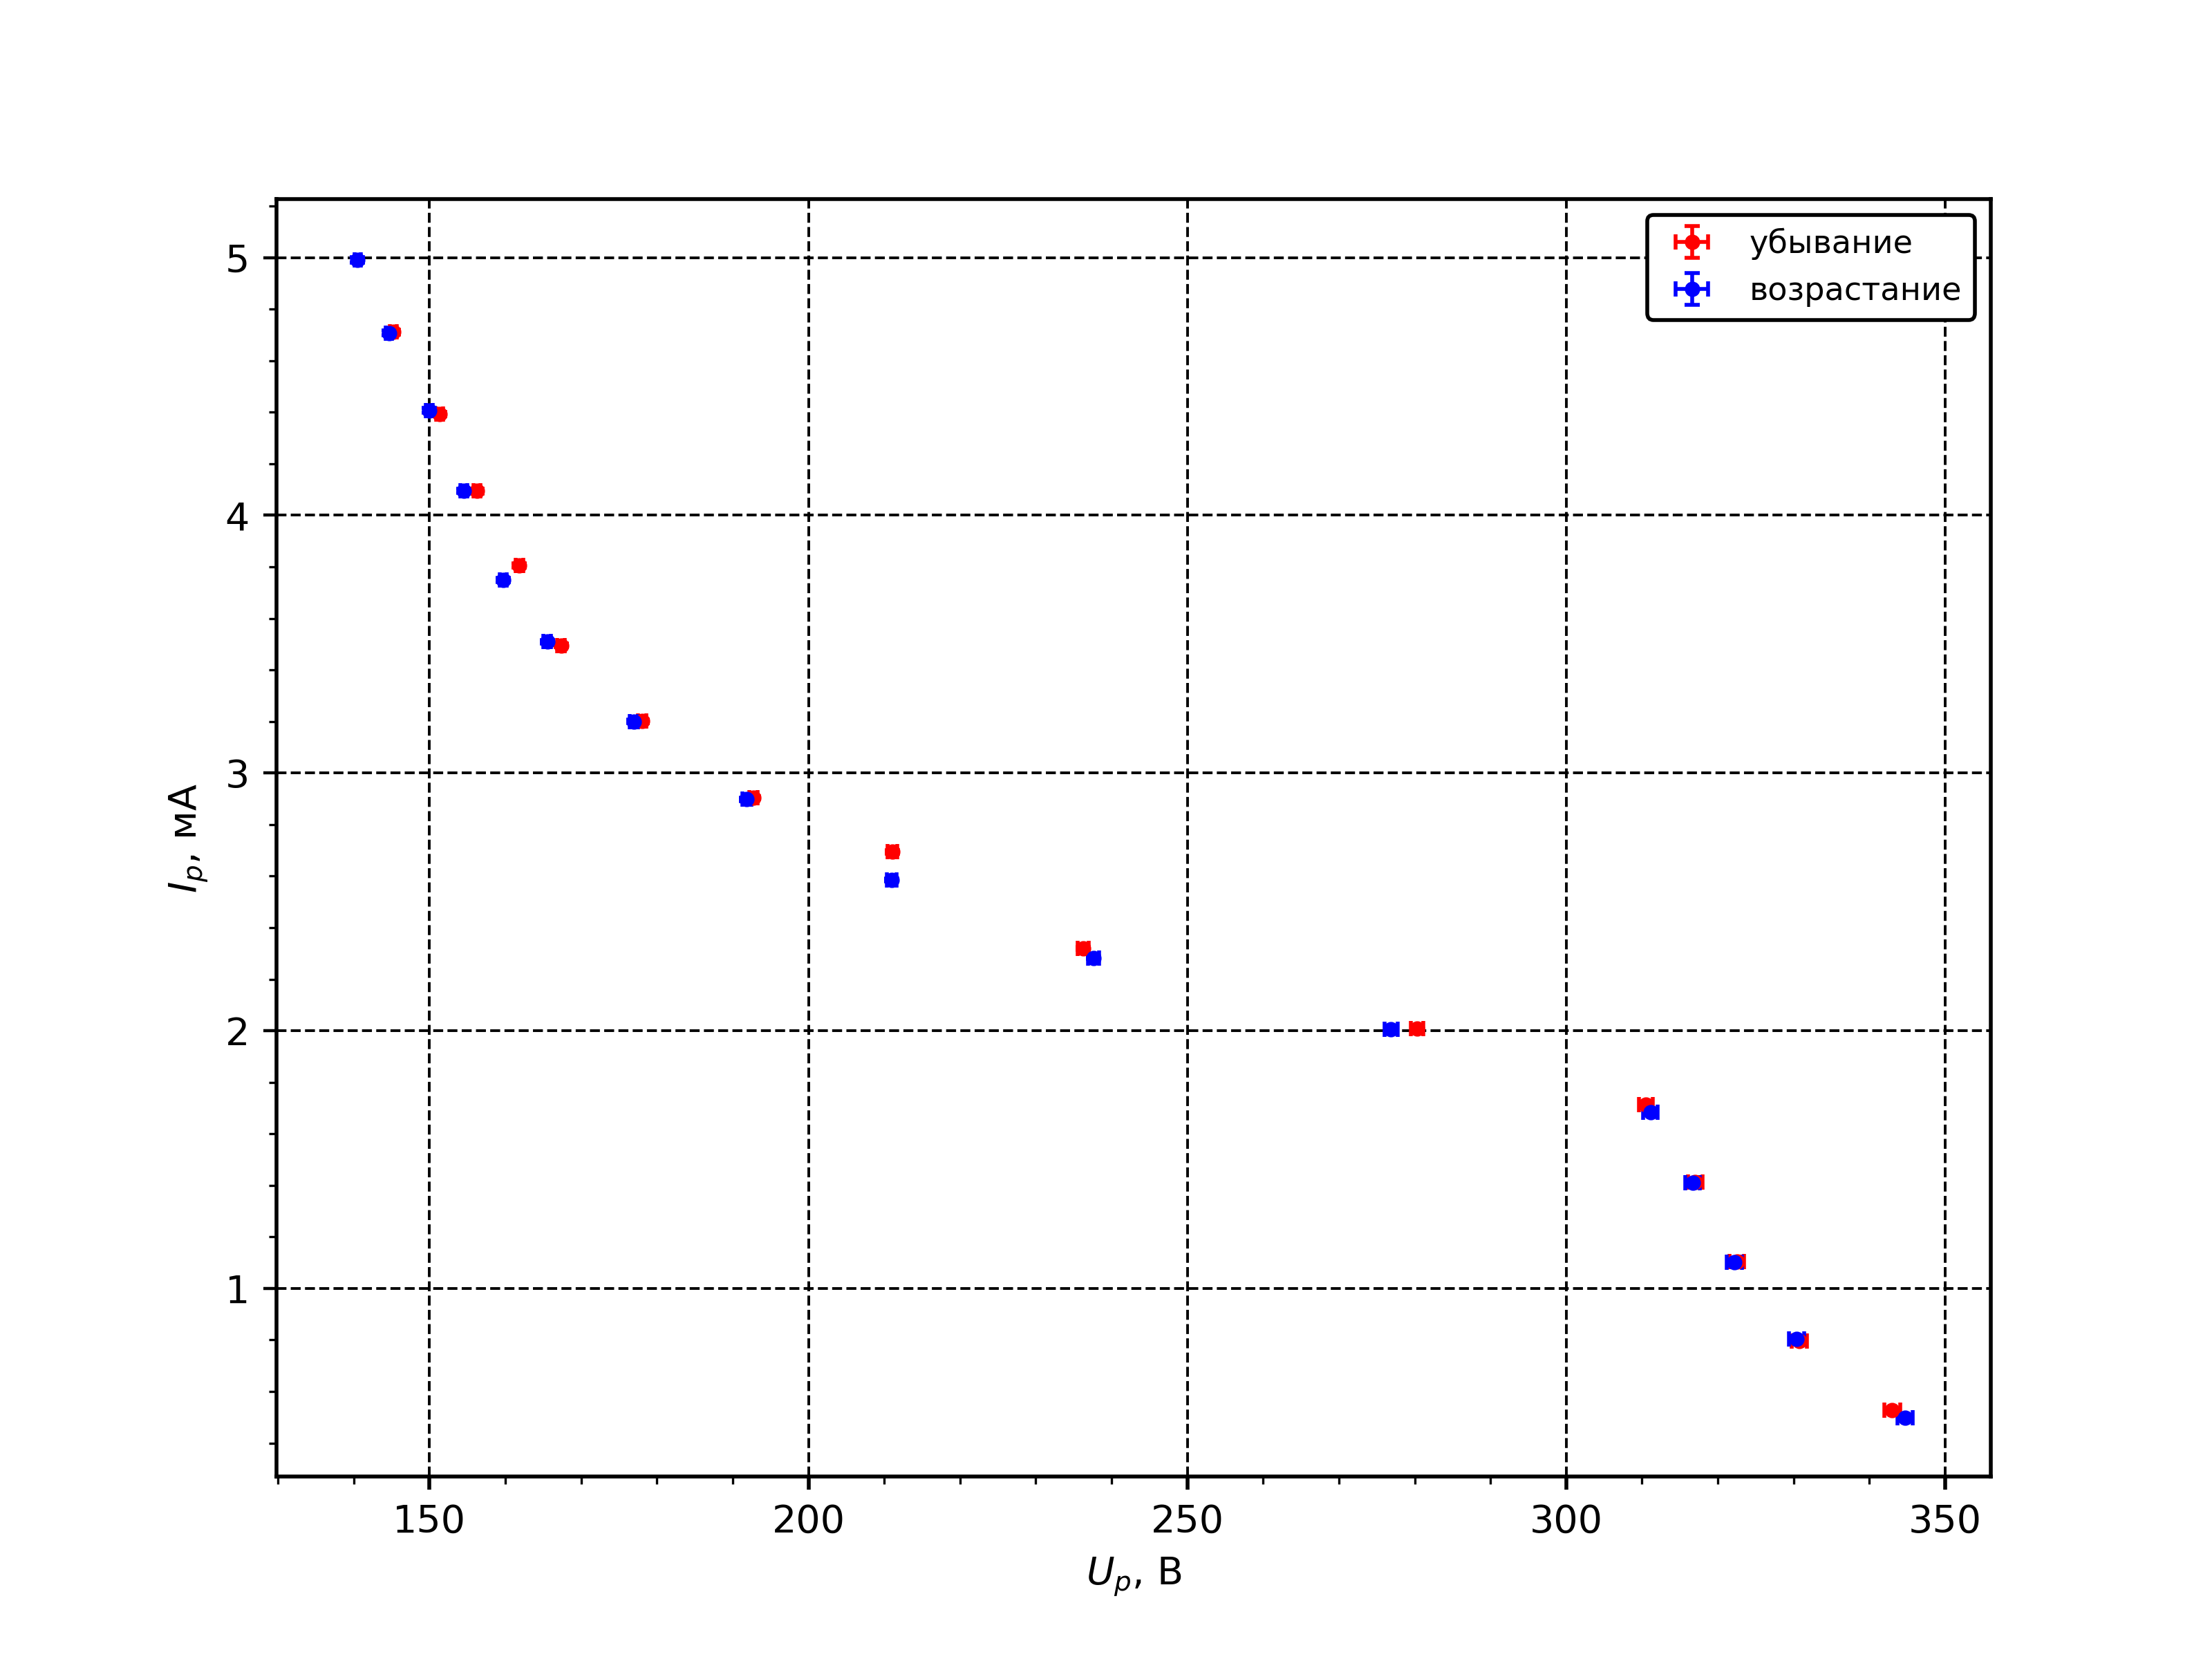
\includegraphics[width=0.8\linewidth]{../img/vah.png}}
\end{figure}
\begin{figure}[ht!]
    \center{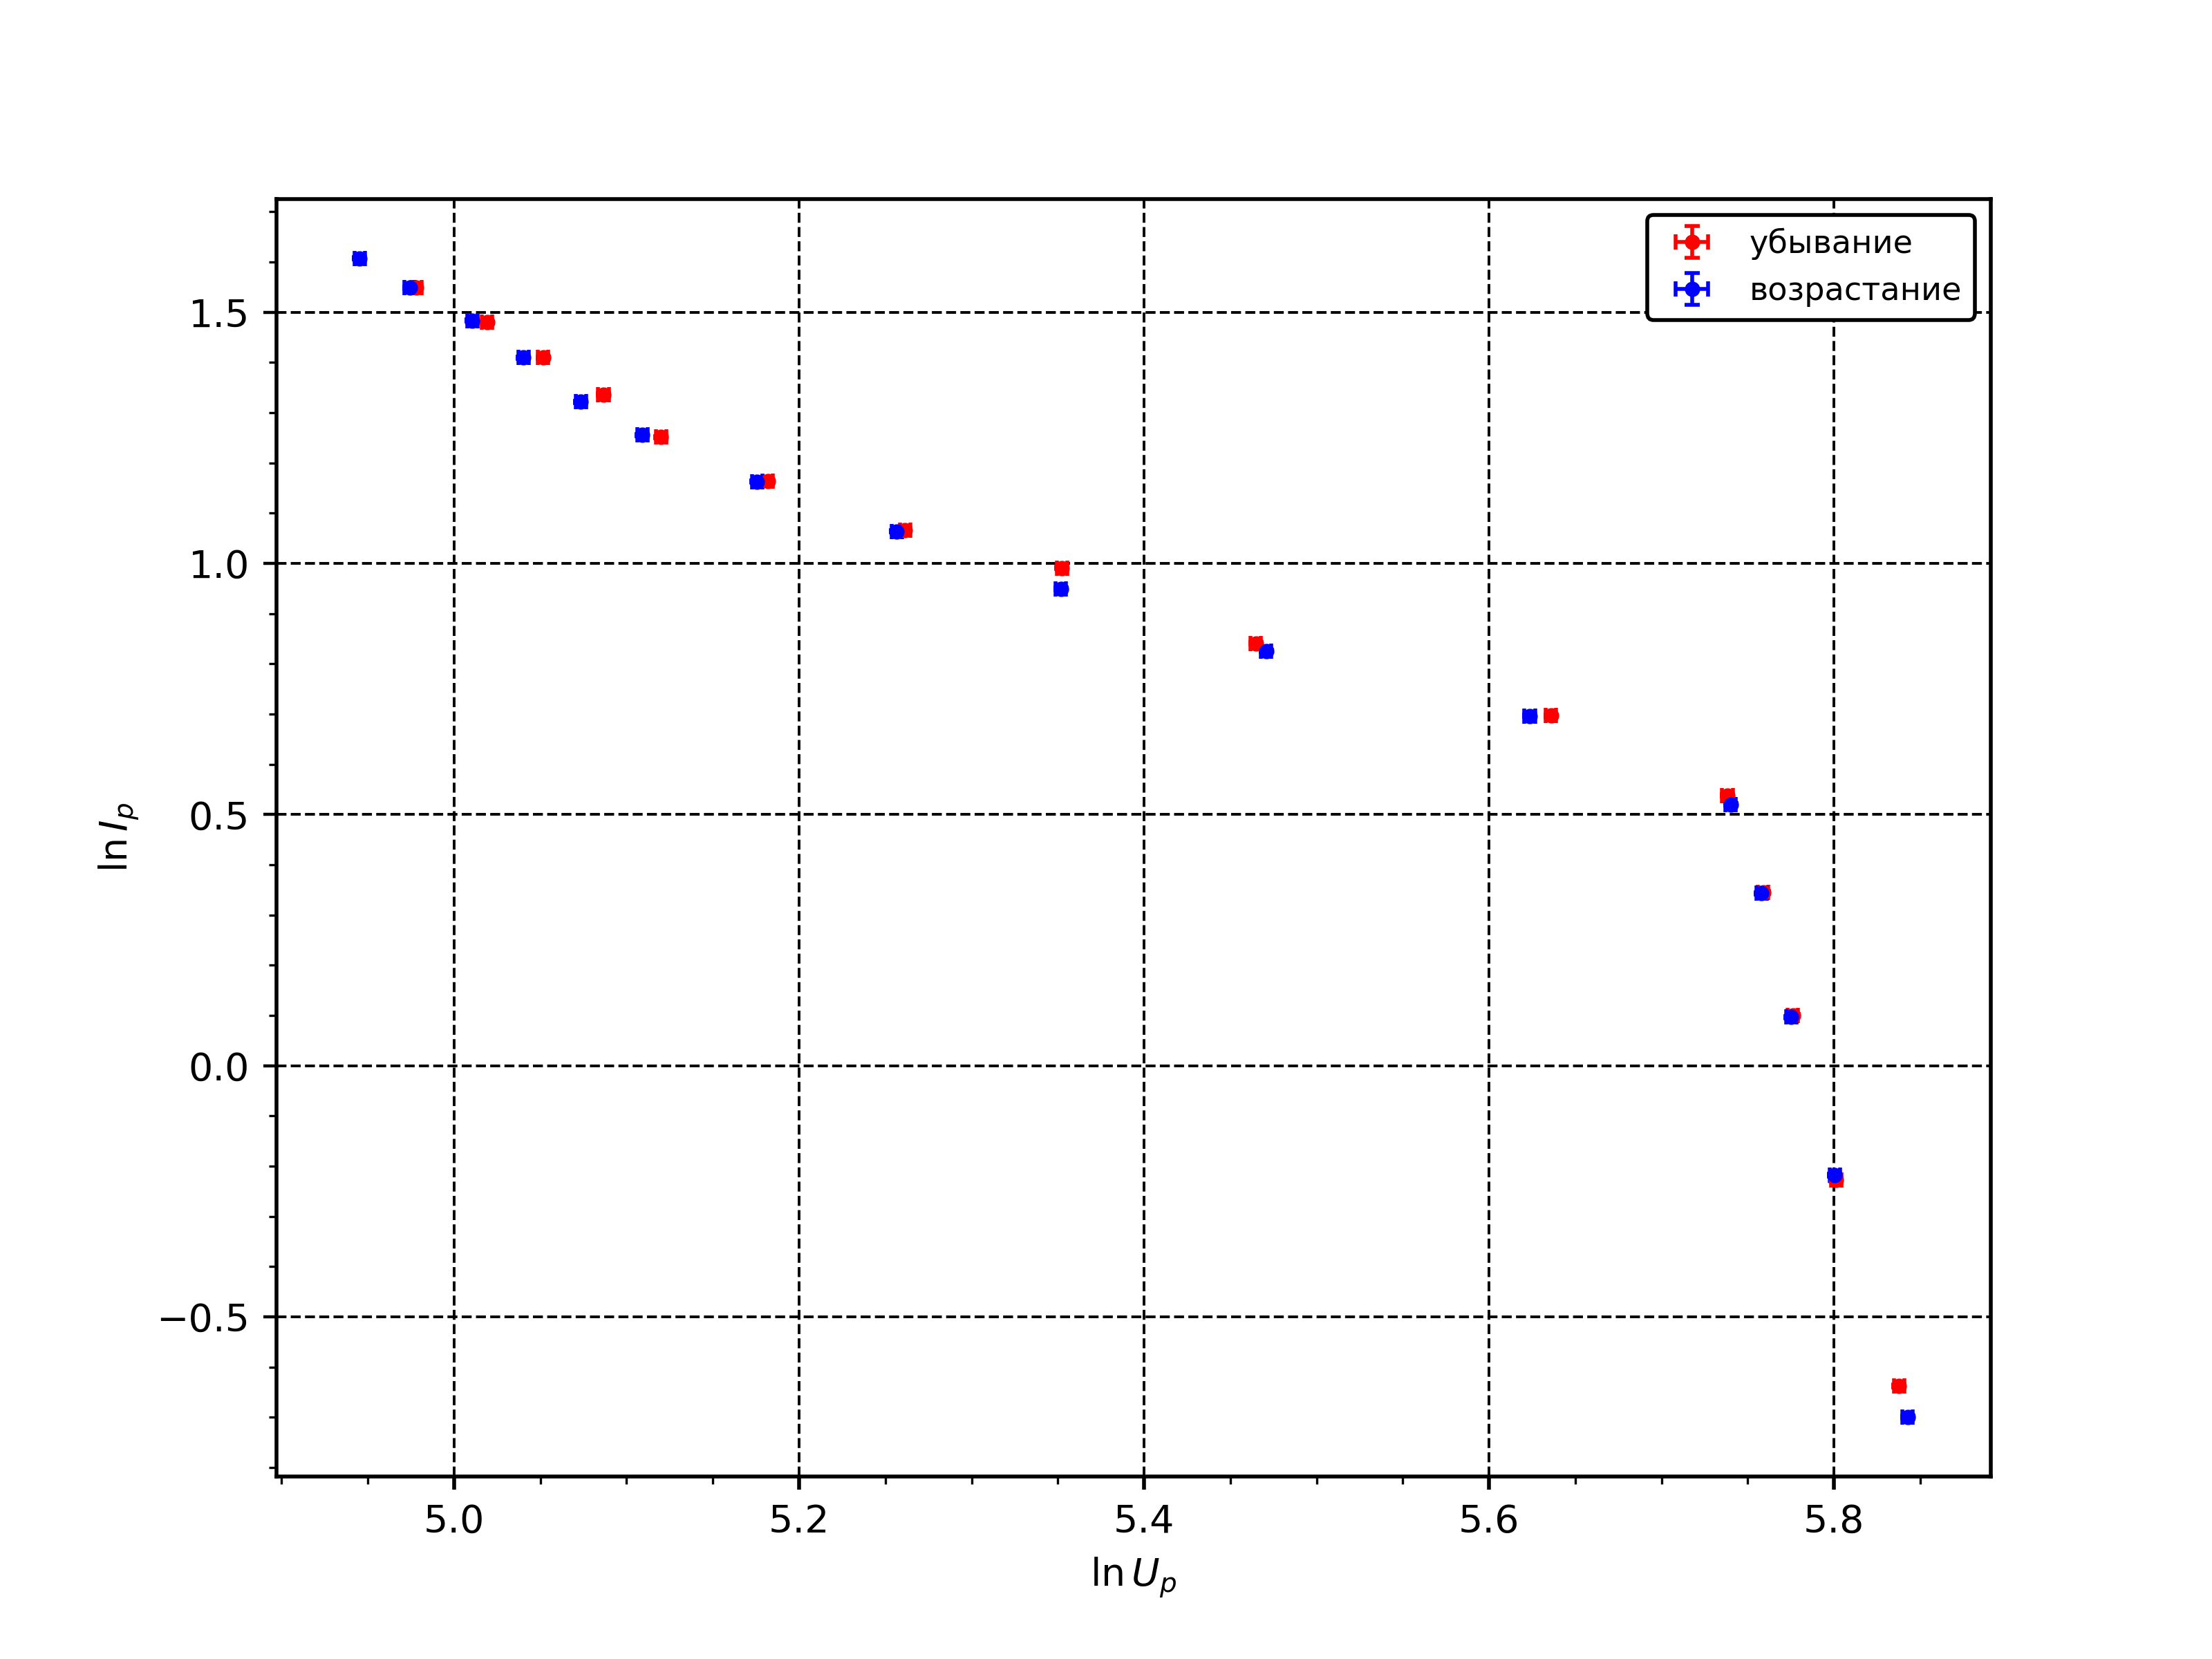
\includegraphics[width=0.8\linewidth]{../img/vah-ln.png}}
\end{figure}
\begin{figure}[ht!]
    \center{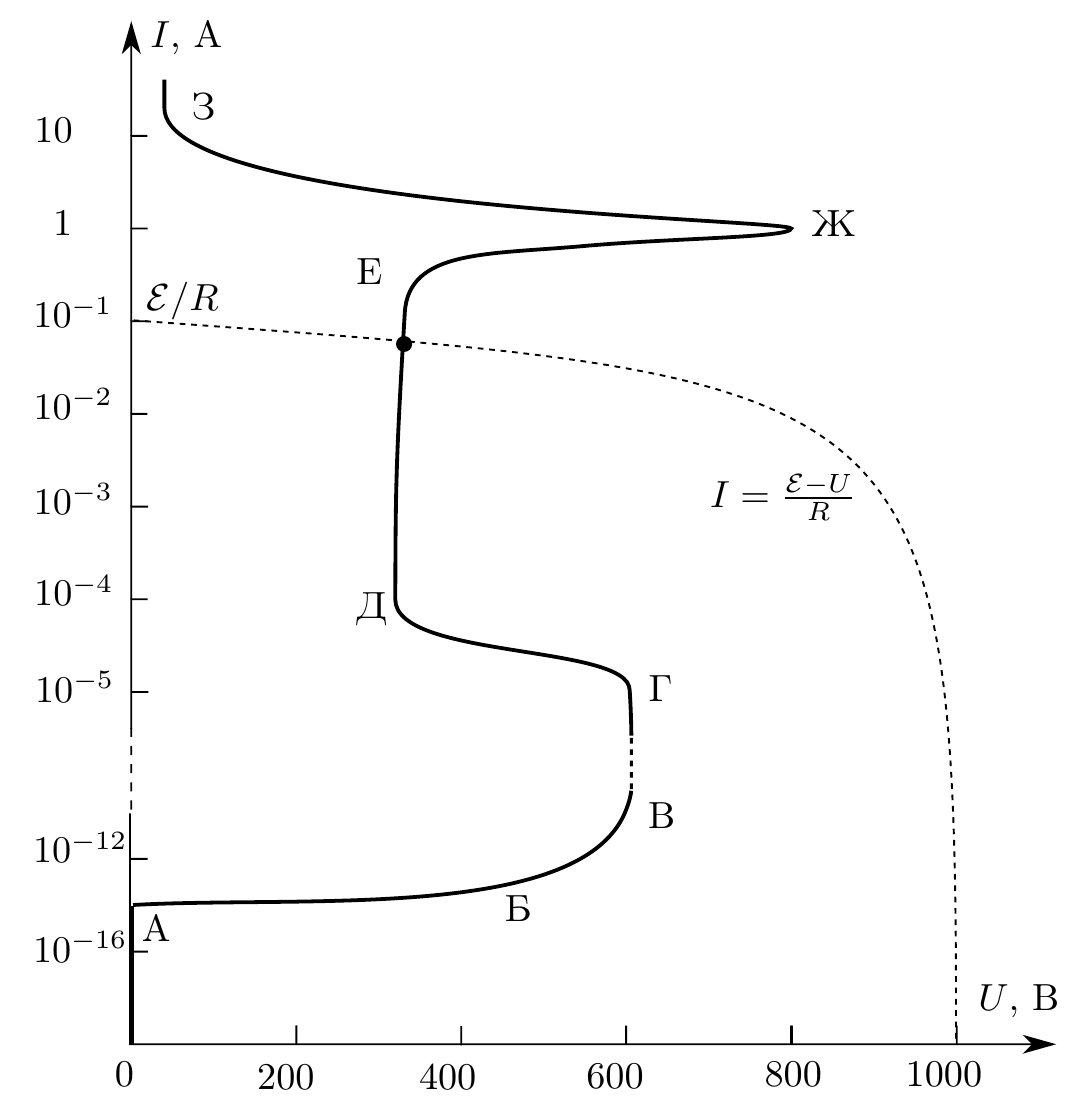
\includegraphics[width=0.5\linewidth]{../img/vah-lol.png}}
\end{figure}

Этот участок ВАХ соответсвтует участку ДГ.

\[
    R_{\text{max}} = \left(-141 \pm 9\right)\cdot 10^{3}\;\text{Ом}
\]

\begin{figure}[ht!]
    \center{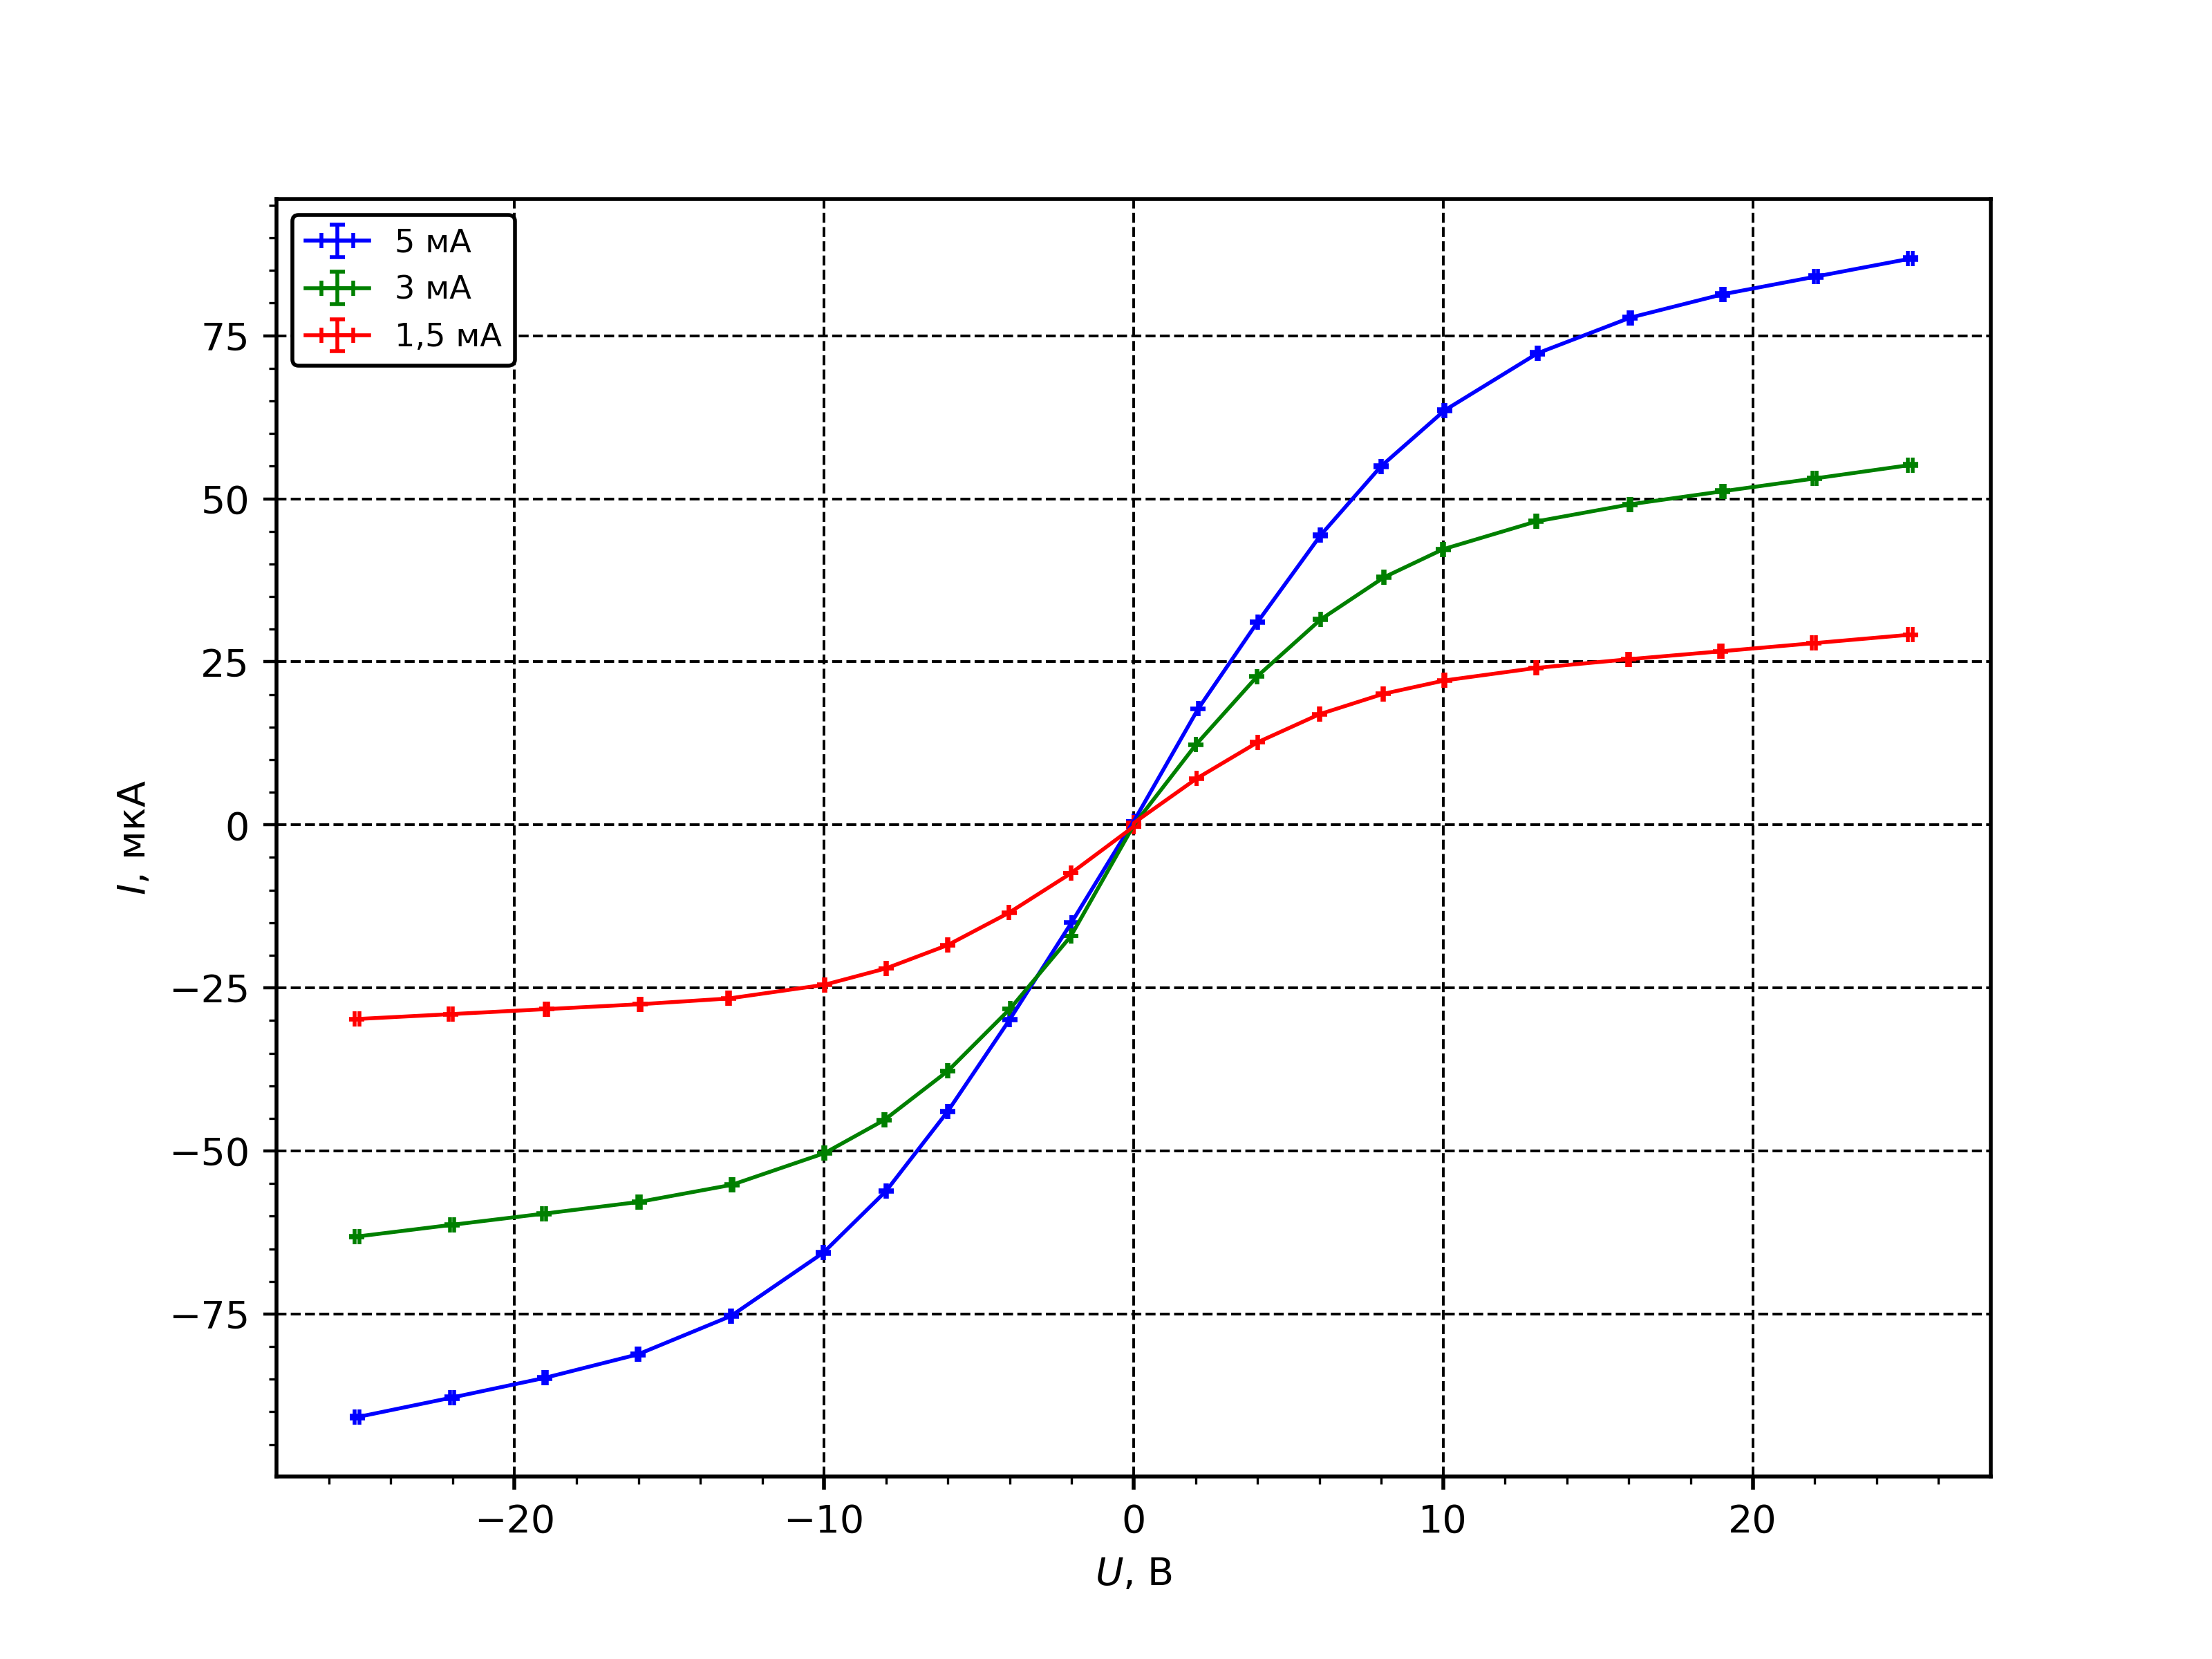
\includegraphics[width=0.8\linewidth]{../img/zh.png}}
\end{figure}

\[
    I_{1{,}5\text{нл}} = 18{,}63 \pm 0{,}07\;\text{мкА} 
\]
\[
    I_{1{,}5\text{нп}} = \left(-23543{,}3 \pm 1{,}5\right)\cdot 10^{-3}\;\text{мкА}
\]
\[
    I_{3\text{нл}} = -47{,}1 \pm 0{,}7\;\text{мкА}
\]
\[
    I_{3\text{нп}} = 38{,}47 \pm 0{,}03\;\text{мкА}
\]
\[
    I_{5\text{нл}} = 58 \pm 2\;\text{мкА}
\]
\[
    I_{5\text{нп}} = -64{,}4 \pm 0{,}8\;\text{мкА}
\]
\[
    I_{1{,}5\text{н}} = 21 \pm 2\;\text{мкА}
\]
\[
    I_{3\text{н}} = 43 \pm 4\;\text{мкА}
\]
\[
    I_{5\text{н}} = 61 \pm 3\;\text{мкА}
\]
\[
    \frac{dI}{dU}_{1{,}5} = 3{,}63 \pm 0{,}09\;\text{мкА} / \text{В}
\]
\[
    \frac{dI}{dU}_{3} = 5{,}8 \pm 0{,}2\;\text{мкА} / \text{В}
\]
\[
    \frac{dI}{dU}_{5} = 8{,}0 \pm 0{,}2\;\text{мкА} / \text{В}
\]

\[
    n_{e} = \frac{2{,}5I_{\text{н}}}{e \pi dl \sqrt{\frac{2kT_{e}}{m_{i}}}}
\]
\[
    T_{e} = \frac{eI_{\text{н}}}{2k\frac{dI}{dU}}
\]
\[
    w_{p} = \sqrt{\frac{4 \pi n_{e} e^{2}}{m_{e}}}
\]
\[
    r_{D_{e}} = \sqrt{\frac{kT_{e}}{4 \pi n_{e} e^{2}}}
\]
\[
    r_{D} = \sqrt{\frac{kT_{i}}{4 \pi n_{e}e^{2}}}
\]
\[
    N_{D} = \frac{4}{3} \pi r_{D}^{3} n_{i}
\]
\[
    \alpha = n_{e} / n
\]
\[
    P = nkT
\]
\[
    T_{e_{1{,}5}} = \left(34 \pm 4\right)\cdot 10^{3}\;\text{К}
\]
\[
    T_{e_{3}} = \left(43 \pm 5\right)\cdot 10^{3}\;\text{К}
\]
\[
    T_{e_{5}} = \left(45 \pm 3\right)\cdot 10^{3}\;\text{К}
\]
\[
    n_{15} = \left(19{,}9 \pm 1{,}2\right)\cdot 10^{15}\;\text{м}^{-3}
\]
\[
    n_{3} = \left(36 \pm 2\right)\cdot 10^{15}\;\text{м}^{-3}
\]
\[
    n_{5} = \left(50{,}3 \pm 1{,}4\right)\cdot 10^{15}\;\text{м}^{-3}
\]
\[
    \omega_{1{,}5} = \left(79 \pm 2\right)\cdot 10^{8}\;\text{с}^{-1}
\]
\[
    \omega_{3} = \left(106 \pm 3\right)\cdot 10^{8}\;\text{с}^{-1}
\]
\[
    \omega_{5} = \left(126 \pm 2\right)\cdot 10^{8}\;\text{с}^{-1}
\]
\[
    r_{D_{e}1{,}5} = \left(85 \pm 3\right)\cdot 10^{-5}\;\text{см}
\]
\[
    r_{D_{e}3} = \left(71 \pm 3\right)\cdot 10^{-5}\;\text{см}
\]
\[
    r_{D_{e}5} = \left(61{,}5 \pm 1{,}2\right)\cdot 10^{-5}\;\text{см}
\]
\[
    r_{D1{,}5} = \left(205 \pm 6\right)\cdot 10^{-6}\;\text{см}
\]
\[
    r_{D3}= \left(152 \pm 4\right)\cdot 10^{-6}\;\text{см}
\]
\[
    r_{D5} = \left(129 \pm 2\right)\cdot 10^{-6}\;\text{см}
\]
\[
    r_{D} \ll 1\;\text{см}
\]
Поэтому плазма квазинейтральна.
\[
    N_{1{,}5} = 0{,}72 \pm 0{,}02
\]
\[
    N_{3} = \left(451 \pm 6\right)\cdot 10^{-3}
\]
\[
    N_{5} = 0{,}533 \pm 0{,}014
\]
\[
    N_{D} \approx 1
\]
поэтому плазма неидеальная.
\[
    \alpha_{1{,}5} = \left(31 \pm 2\right)\cdot 10^{-8}
\]
\[
    \alpha_{3} = \left(78 \pm 2\right)\cdot 10^{-8}
\]
\[
    \alpha_{5} = \left(56 \pm 3\right)\cdot 10^{-8}
\]

\begin{figure}[ht!]
    \center{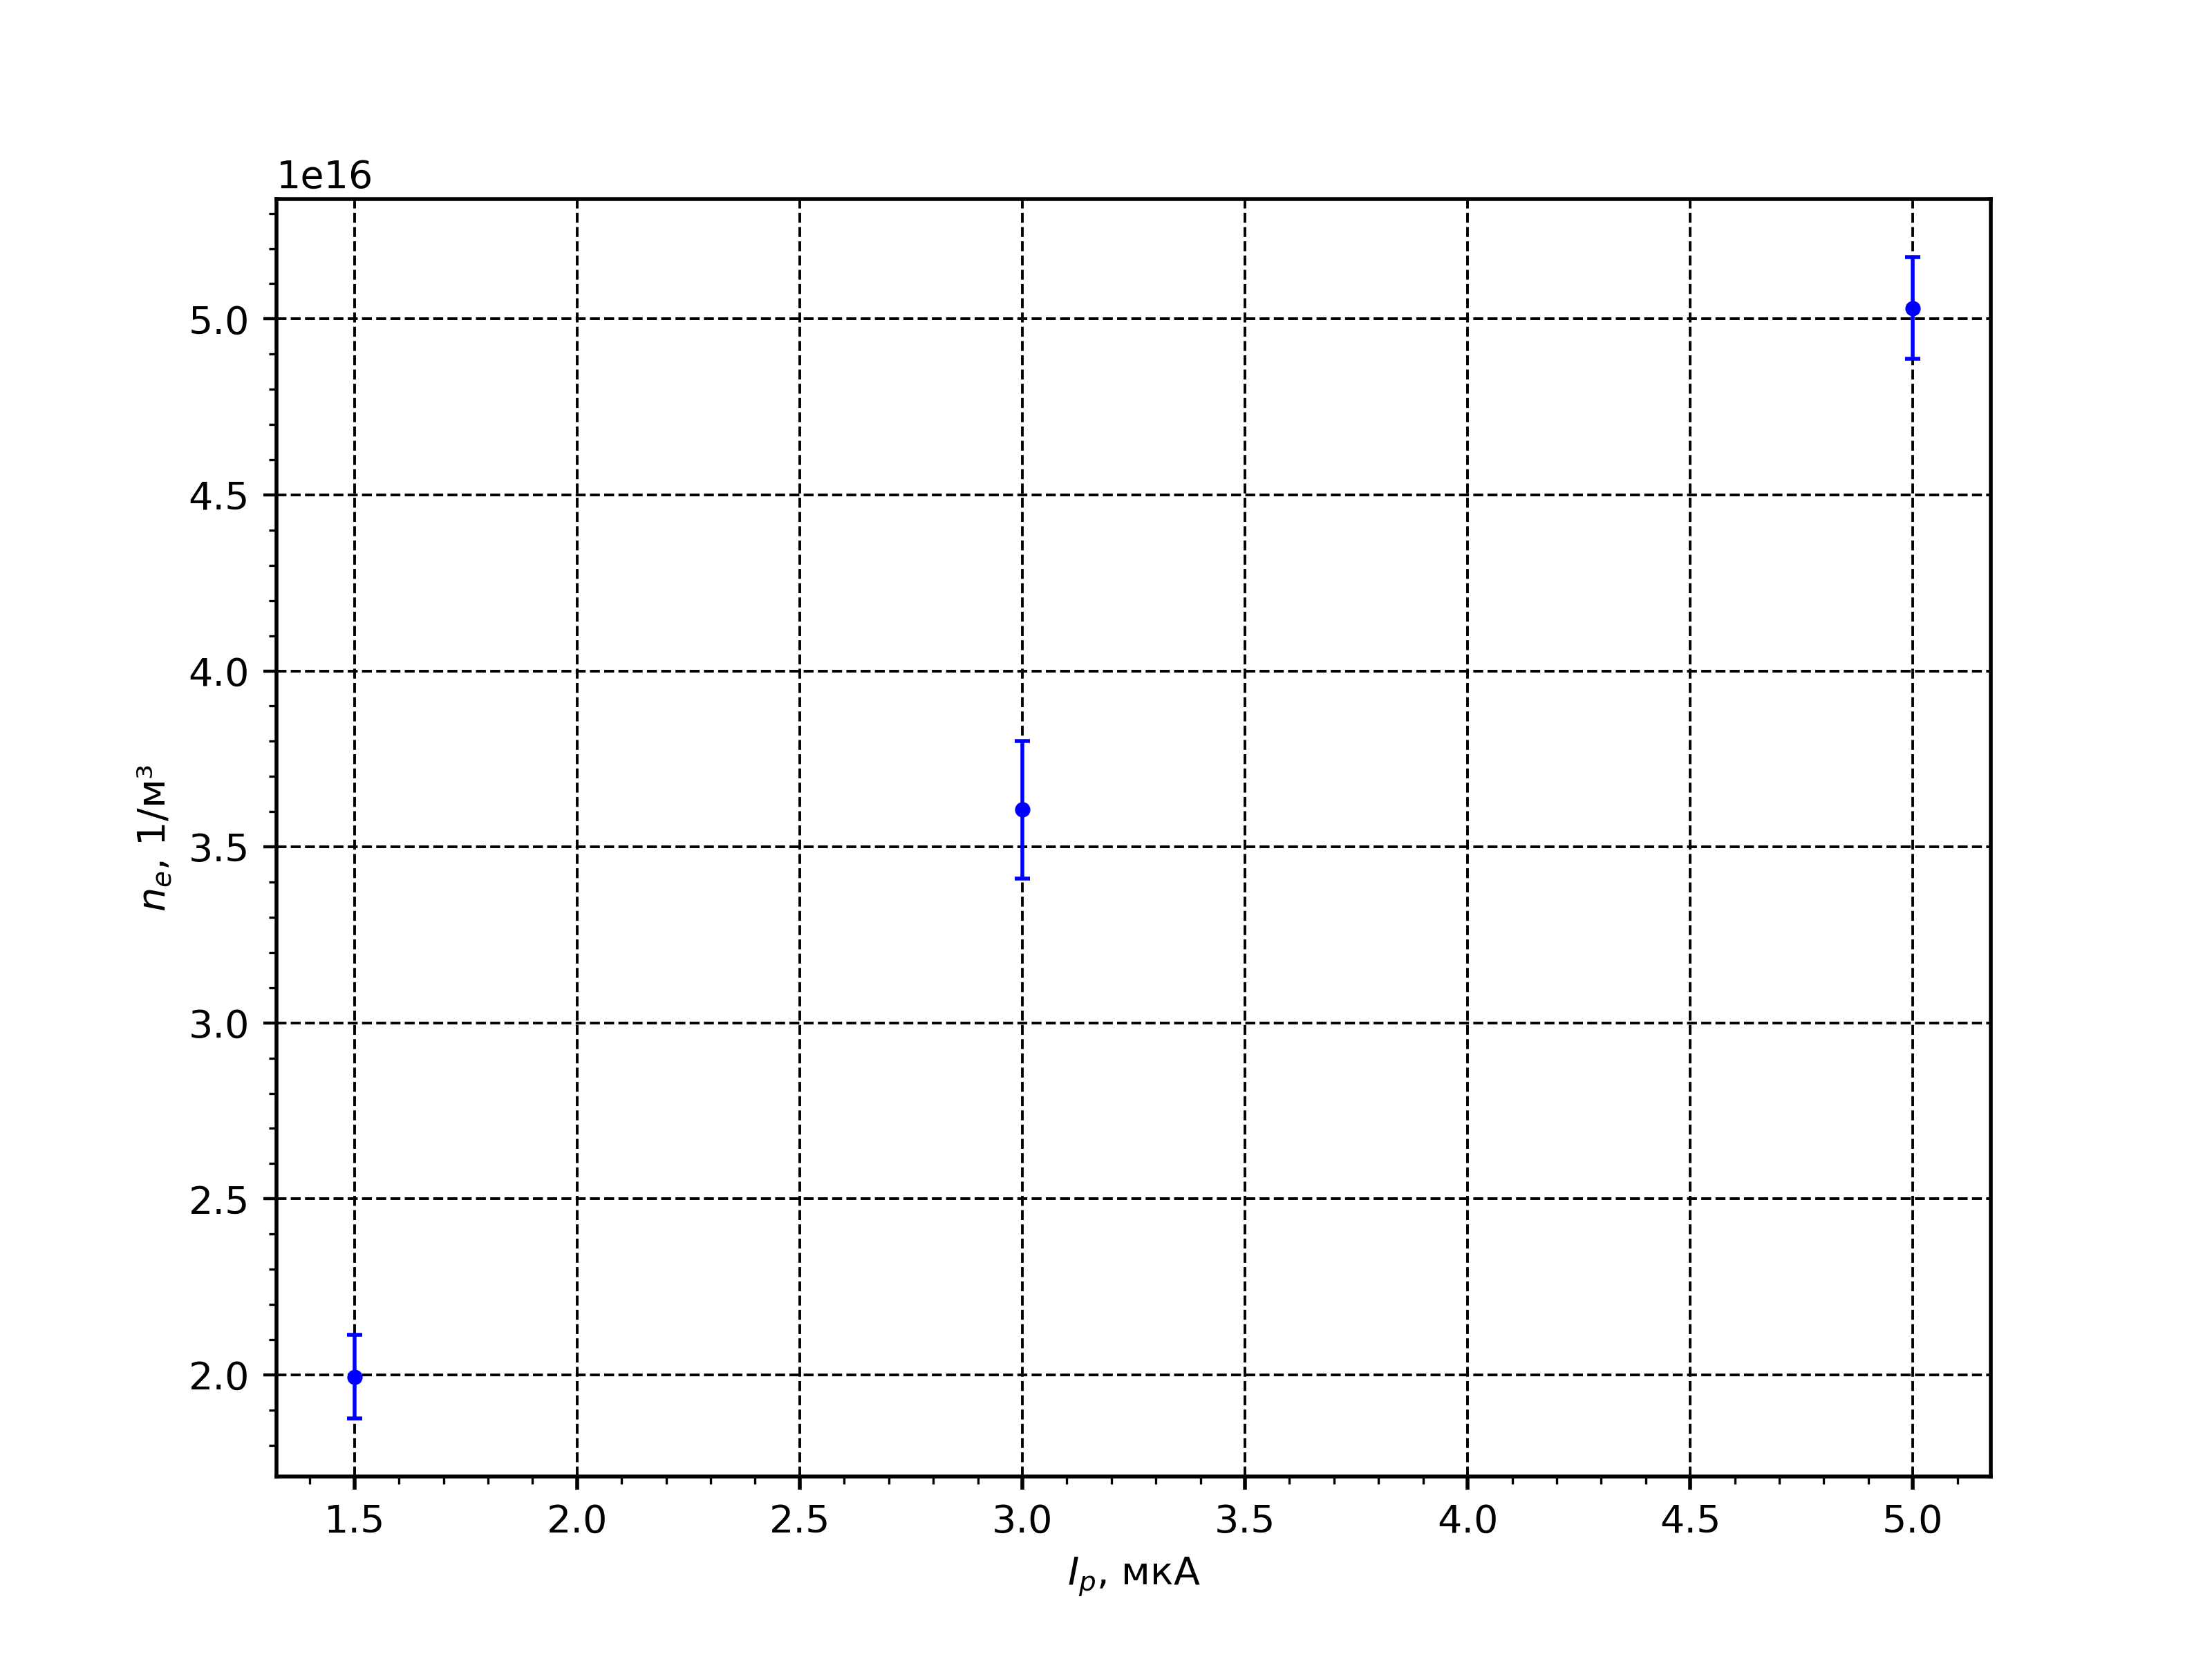
\includegraphics[width=0.8\linewidth]{../img/ni.png}}
\end{figure}
\begin{figure}[ht!]
    \center{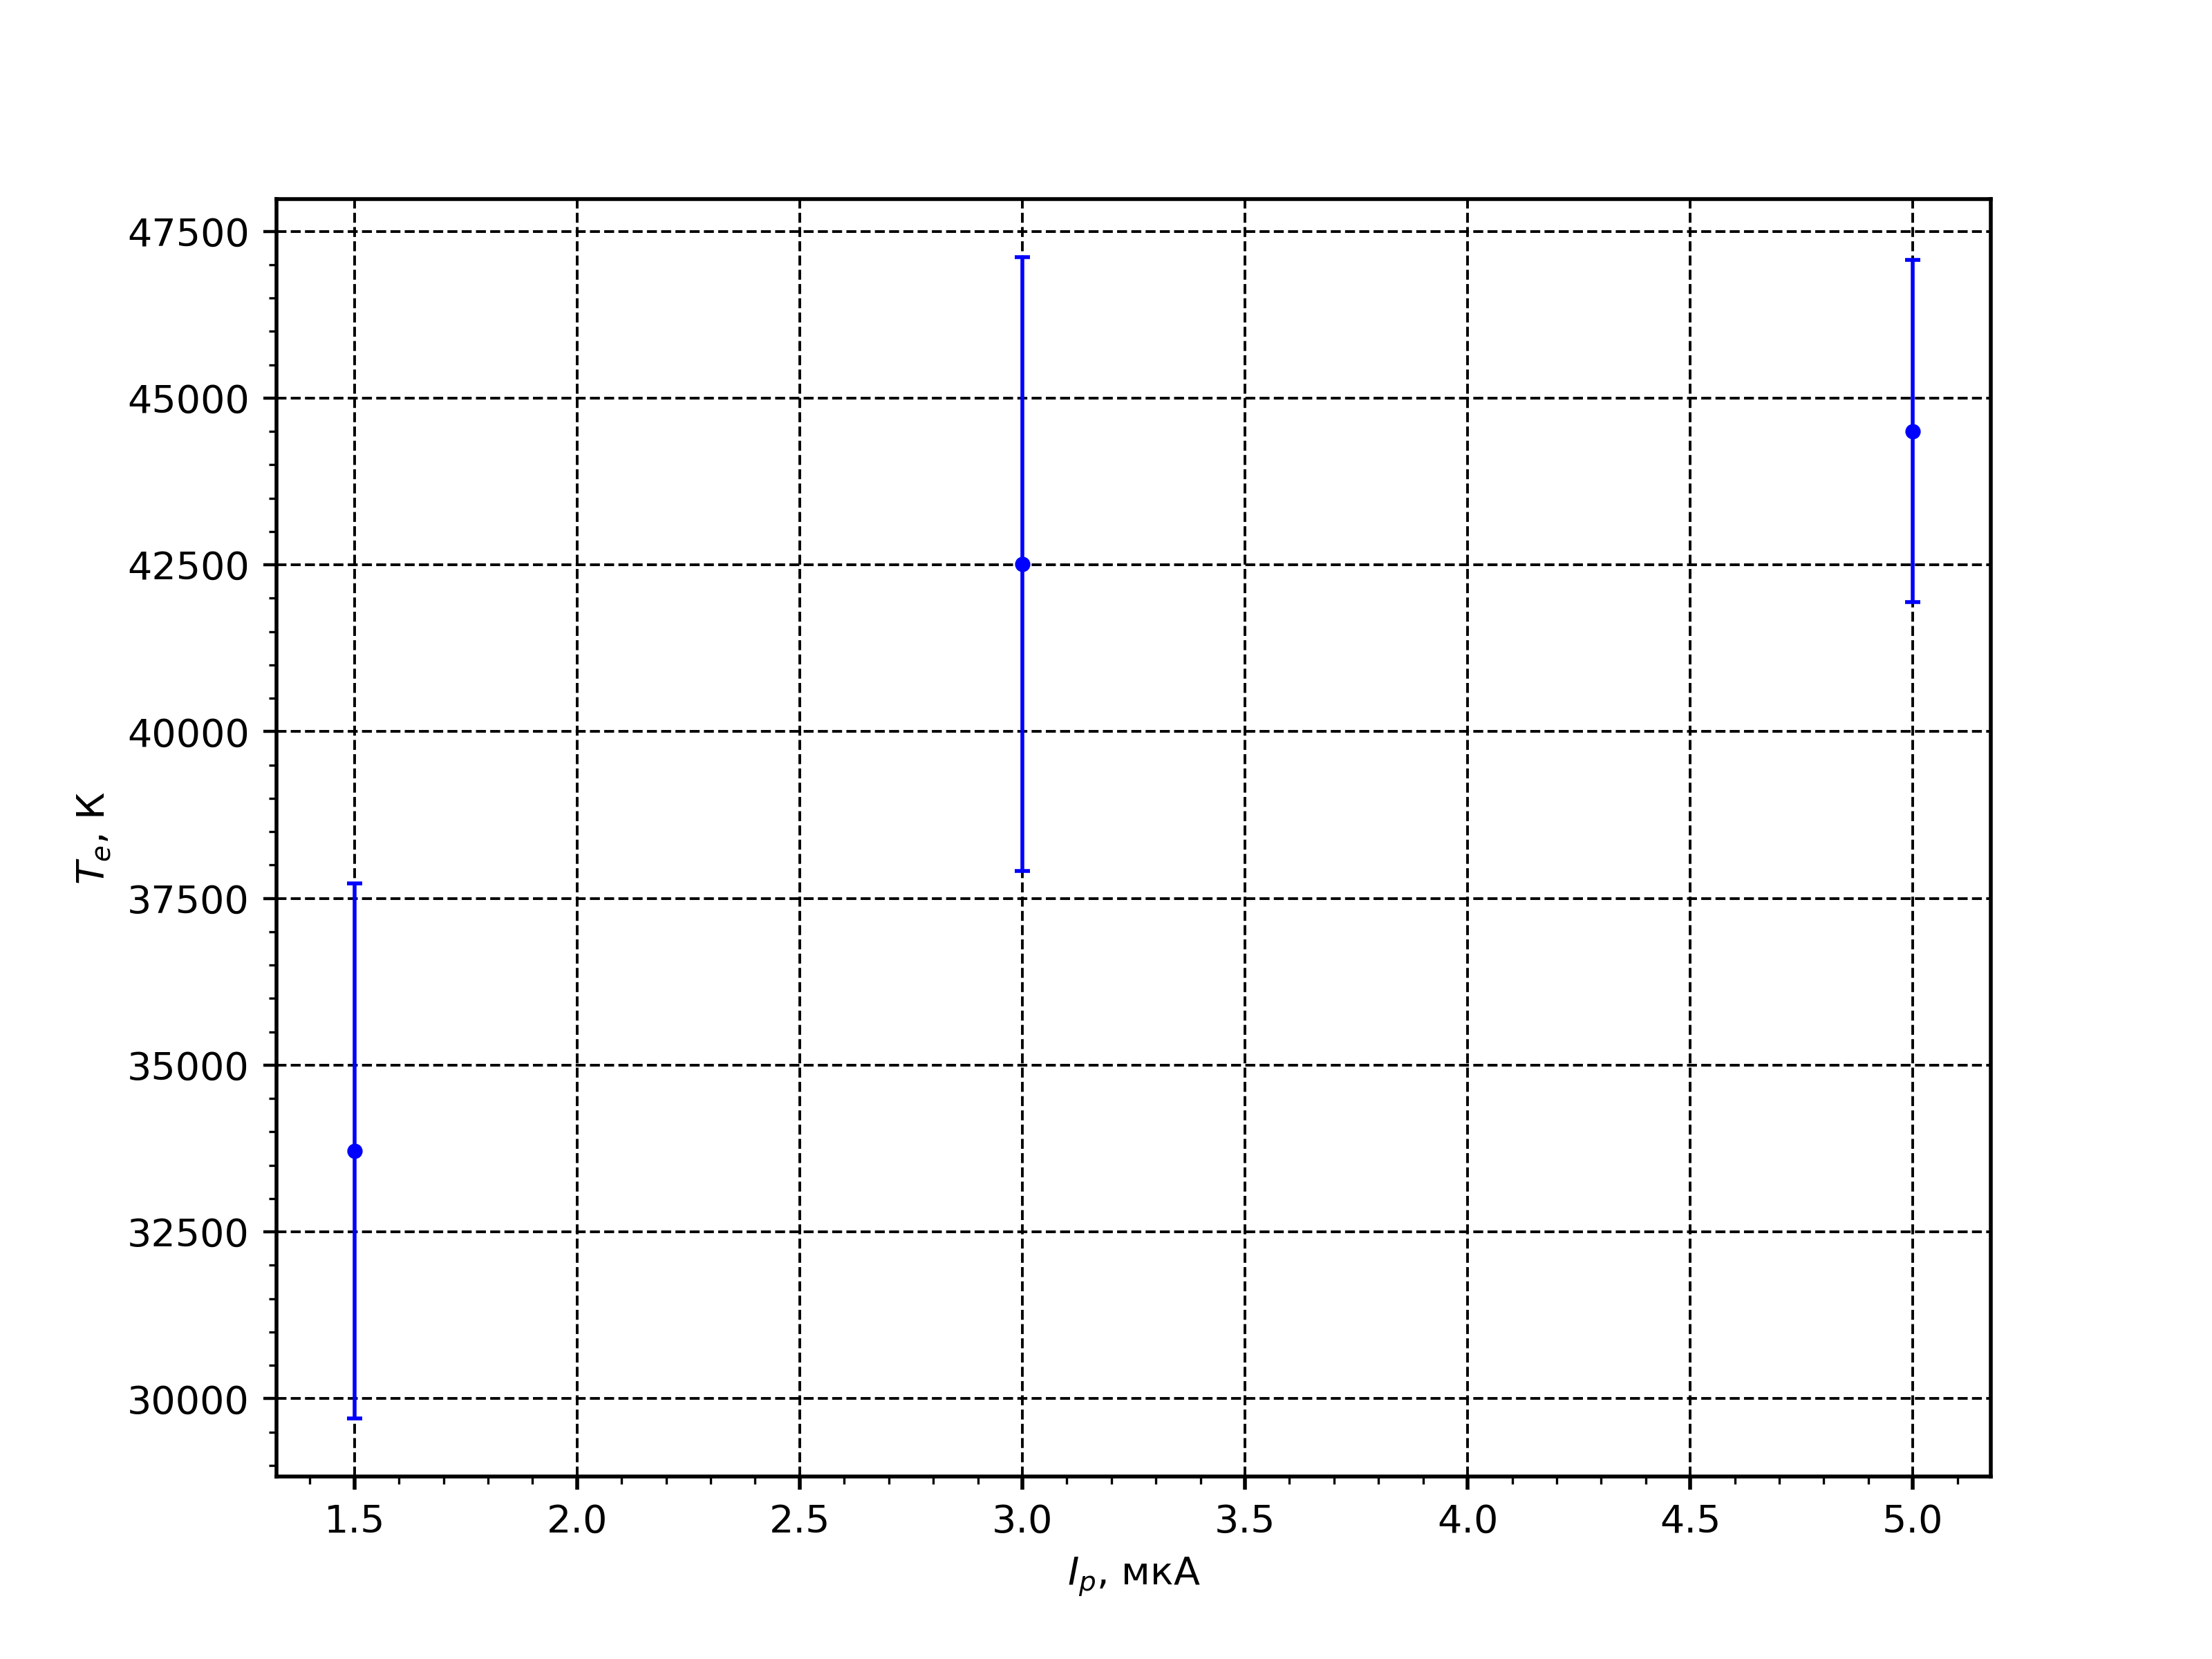
\includegraphics[width=0.8\linewidth]{../img/ti.png}}
\end{figure}
Энергия электронов и их концентрация либо одновременно растут, либо одновременно падают (т.к. с ростом энергии растет вероятность того, что электрон ионизирует атом и наоборот). При этом если они одновременно падают, то и ток должен уменьшиться. Поэтому они одновременно растут.

Концентрация электронов от времени растет линейно с хорошей точностью. О виде зависимости энергии электронов от тока говорить сложно из-за больших погрешностей и малого числа точек.
